\chapter{Optimisation results}
\label{chap:optimisation-results}

Testing the impact of my optimisations presents three primary
difficulties:

\begin{enumerate}
\item The optimisation is ``incomplete'', in the sense that we likely
  fuse too aggressively (as outlined in \cref{sec:whentofuse}), and
  are too conservative about duplicating trivial computation.

\item There is not yet a way to execute \LO{} code in a performant
  manner.  The \LO{} compiler has an interpreter, but its performance
  characteristics are very different from parallel hardware -- for
  example, variable bindings carry great overhead.

  The compiler also has a code generator which generates strictly
  sequential C code.  The resulting C code uses very naïve memory
  management, however.  In particular it copies arrays very often when
  entering loops, although this might put the fusion optimisation in a
  better light, as it will reduce the sum number of loops.

\item Finally, fusion, which is our primary optimisation, does not
  really reduce the number of discrete computation steps necessary to
  execute the program.  The purpose of our fusion optimisation is to
  increase parallelism and reduce the number of discrete GPU kernels,
  which is not something that will benefit the sequential code
  generated by our code generator.
\end{enumerate}

Nevertheless, I will make an attempt at evaluating the impact of the
fusion optimisation.  This will primarily be in the form of manual
inspection of program structure befor and after optimisation, with
comments on the quality of the result.  The reader can be assured that
said inspection of hundreds of lines of machine-generated code was
enormously tedious.

Six programs will be used for evaluation: three relatively simple,
artificial benchmarks, and three real-world financial programs that
have been manually translated from C++ to what we consider
``idiomatic'' \LO{}\footnote{Or at least as much as it makes sense to
  talk about an ``idiomatic'' style for a language whose users are its
  designers.}.  I present runtimes for these programs in
\cref{sec:runtime-results}.

The code for the artificial benchmarks can be found in
\cref{app:artificial-benchmark-programs}, as well as the programs
resulting from optimisation, but are summarised here:

\begin{description}
% data/benchmarks/BlackScholes.l0
\item[P0] Black-Scholes\cite{black1973pricing} pricing computation.
  34 SLOC (Source Lines Of Code - ignoring comments and blank lines).

% data/tests/MatMultFun.l0
\item[P1] Matrix multiplication written in a functional style (i.e, no
  use of \texttt{loop} and \texttt{let-with}).  13 SLOC.

% data/benchmarks/BabyBear.l0
\item[P2] BabyBear - a tiny ursine.  27 SLOC.
\end{description}

And the real world benchmarks:

\begin{description}
% data/benchmarks/PricingLexiFi.l0
\item[R0] Pricing program.  344 SLOC.

% data/benchmarks/HiperfitEgCos.l0
\item[R1] Some C++ mess we got from Nordea.  172 SLOC.

% data/benchmarks/CalibLexiFi.l0
\item[R2] Parameter calibration program.  798 SLOC.

\end{description}

\begin{figure}
\begin{tabular}{p{1.6cm}|p{1.6cm}|p{1.6cm}|p{1.6cm}|p{1.6cm}|p{1.6cm}}
\multicolumn{2}{c}{\textbf{P0}} & \multicolumn{2}{c}{\textbf{P1}} & \multicolumn{2}{c}{\textbf{P2}} \\
\hline
Before & After & Before & After & Before & After \\
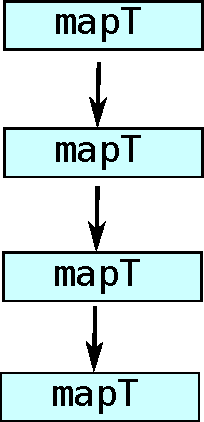
\includegraphics[width=1.6cm]{img/BlackScholes-unfused.pdf} &
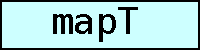
\includegraphics[width=1.6cm]{img/BlackScholes-fused.pdf} &
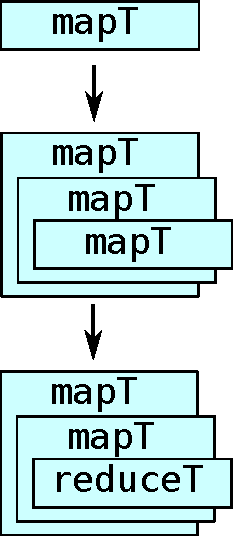
\includegraphics[width=1.6cm]{img/MatMultFun-unfused.pdf} &
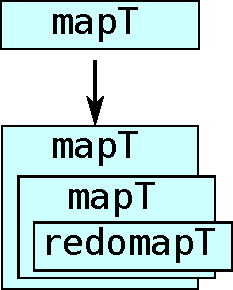
\includegraphics[width=1.6cm]{img/MatMultFun-fused.pdf} &
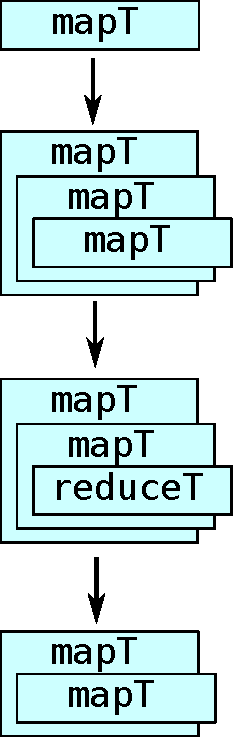
\includegraphics[width=1.6cm]{img/BabyBear-unfused.pdf} &
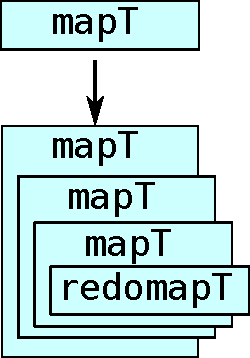
\includegraphics[width=1.6cm]{img/BabyBear-fused.pdf}
\end{tabular}
\caption{Artificial benchmark dataflows, before and after optimisation}
\label{fig:artificial-dataflows}
\end{figure}

The structure of the artificial benchmarks are shown on
\cref{fig:artificial-dataflows}.  P0, being a straightforward sequence
of four \texttt{map}s, fuses well.  P1 also fuses well - the main loop
becomes a two-dimensional \texttt{tmap}, with the dot product at each
location being computed in a \texttt{redomap}.  Although not visible
in the data flow diagram, it is worth remarking that hoisting has
moved all \texttt{assert} expressions (originating in the use of
\texttt{zip}) out of the main loop, which can thus be evaluated with
no bounds checking - or indeed, any branching at all.

There is clearly a missed opportunity for fusion, though, the reason
for which becomes clear when we inspect the code around the unfused
\texttt{map}:
\begin{colorcode}
..
let {untuple_13} =
  mapT(fn \{[[int]]\} ([int] param_0_8) =>
         // tmp_repl_11 aliases param_0_8
         let tmp_repl_11 = replicate(N_2, param_0_8) in
         \{tmp_repl_11\},
       x_0) in
let tmp_size_14 = size(2, untuple_13) in
... // untuple_13 is eventually input to main loop.
\end{colorcode}
The size analyser is not smart enough to rewrite the \texttt{size}
expression, and \texttt{untuple\_13} is thus used several times,
blocking fusion.  The most reasonable solution is to improve the size
analyser, for which I will outline a potential approach in
\cref{sec:future-work}.  P2 suffers from the same problem, although
again the main loop is nicely fused.

\begin{figure}
\begin{center}
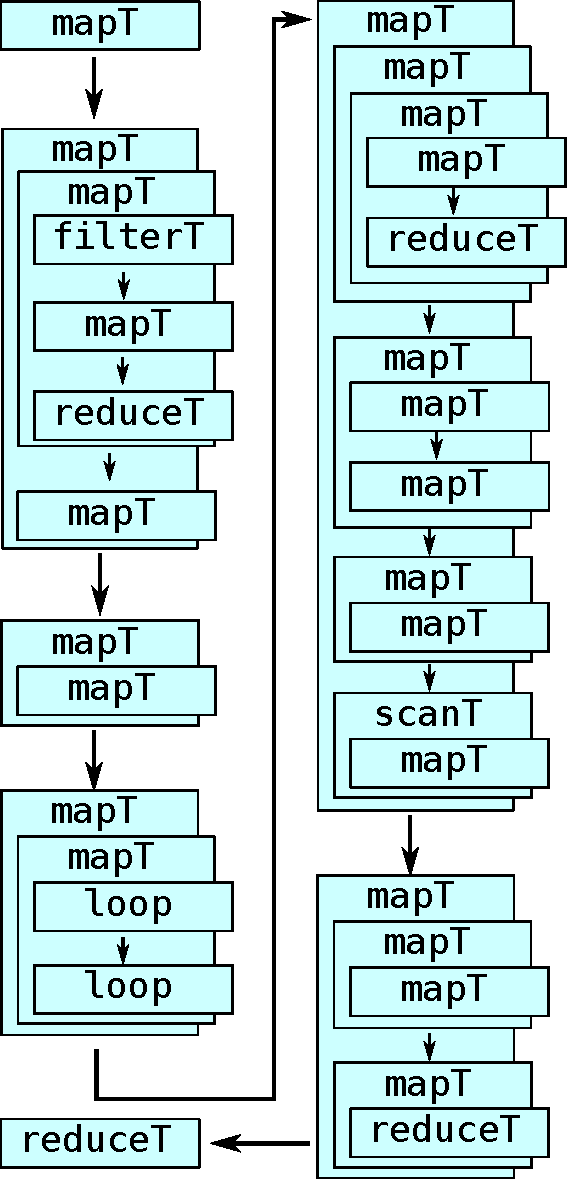
\includegraphics[width=3.2cm]{img/PricingLexiFi-unfused.pdf}
\hspace{1cm}
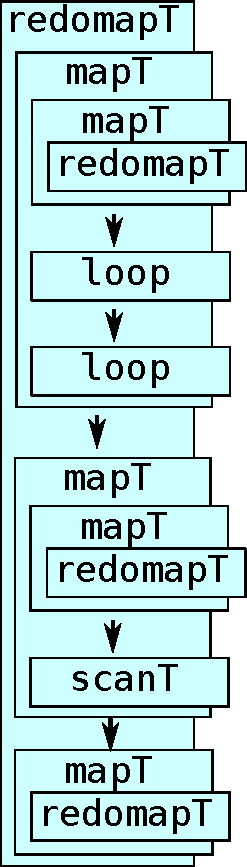
\includegraphics[width=1.6cm]{img/PricingLexiFi-fused.pdf}
\end{center}
\caption{R0 benchmark dataflow, before and after optimisation}
\label{fig:r0-dataflow}
\end{figure}

When illustrating the dataflow for the real-world benchmarks, I
performed some minor simplications.  Specifically, I removed prologue
and epilogue code, in order to emphasise the main loop.

Of the real-world benchmarks, R0, whose dataflow is illustrated on
\cref{fig:r0-dataflow}, benefits the most from optimisations.  The
program is turned into a big \texttt{redomapT} that runs over an array
of a thousand elements.  The body of the \texttt{redomapT} runs three
loops in sequence.  The two first could in principle be fused, but we
are again foiled by limitations of the size analyser.  In this case,
the use of an explitit \texttt{loop} prevents the size analyser from
determining the column size of the two-dimensional array returned by
the \texttt{mapT}.

\begin{figure}
\begin{center}
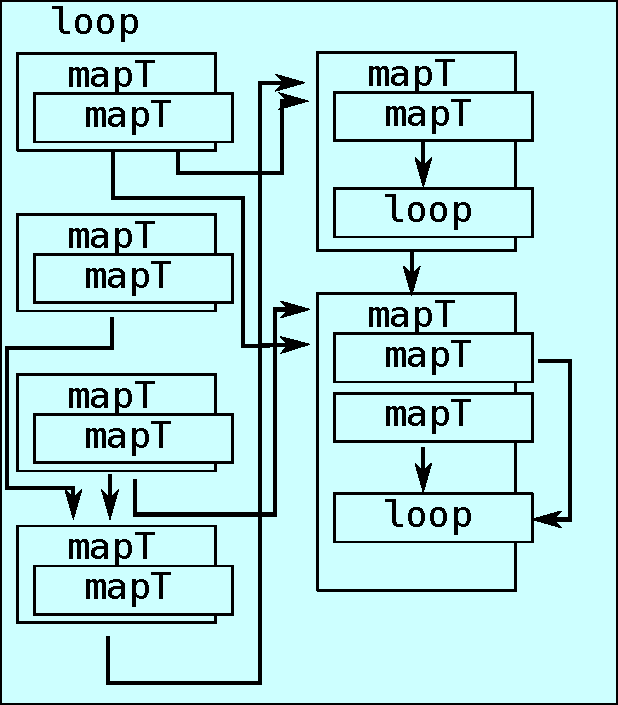
\includegraphics[width=3.2cm]{img/HiperfitEgCos-unfused.pdf}
\hspace{1cm}
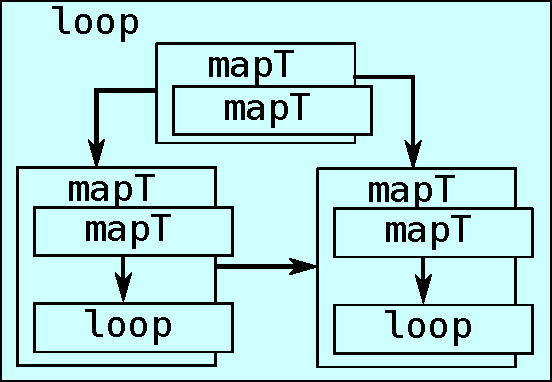
\includegraphics[width=3.2cm]{img/HiperfitEgCos-fused.pdf}
\end{center}
\caption{R1 benchmark dataflow, before and after optimisation}
\label{fig:r1-dataflow}
\end{figure}

For R1, the gains are more muted.  The overall structure is a
sequential, iterative main loop, which of course limits what we can
do, but the body of this loop can in principle be parallelised.  The
unoptimised and optimised loop bodies can be seen on
\cref{fig:r1-dataflow}.  At first sight, two possible avenues for
further fusion are possible:

\begin{enumerate}
\item The first \texttt{mapT} could be fused into its two consumers.
  While this would surely duplicate computation, perhaps it is
  worthwhile in this case.  Inspecting the code, which is shown in
  \cref{fig:r1-unfused-map}, we find that the computation that would
  be duplicated for each element is approximately four primitive
  arithmetic operations, and two calls to exponent and logarithm
  functions.  Such duplication would likely be acceptable if it
  increases the degree of parallelism.

\item The reason for why the two \texttt{loop}-containing
  \texttt{mapT}s are not fused is more tricky.  Although not expressed
  in the diagram, the input to the consumer is \textit{transposed},
  and we have no fusion rule capable of handling a transposition in
  this case, as neither consumer nor producer is a map nest.

  It is not immediately clear how this could be solved.
\end{enumerate}

\begin{figure}
\begin{bcolorcode}
mapT(fn {*[real], *[real], *[real], *[real]} (real xi_481) =>
       let tmp_call_488 = log(xi_481) in
       let bop_493 = 0.5 * tmp_call_488 in
       let {soac_v_506, soac_v_507, soac_v_508, soac_v_509} =
         mapT(fn {real, real, real, real} (real yj_495) =>
                let bop_496 = bop_493 + yj_495 in
                let bop_498 = bop_496 - bop_477 in
                let val_504 = 2.0 * bop_498 in
                let tmp_call_505 = exp(val_504) in
                {0.0, tmp_call_505, 0.0, 0.36},
              untuple_247) in
       {soac_v_506, soac_v_507, soac_v_508, soac_v_509},
     untuple_130)
\end{bcolorcode}
\caption{Unfused map in R1}
\label{fig:r1-unfused-map}
\end{figure}

R2 is next, and that's where things get really ugly.  I'm not saying
anymore about this for now. \fixme{Say more about this.}

\begin{figure}
\begin{center}
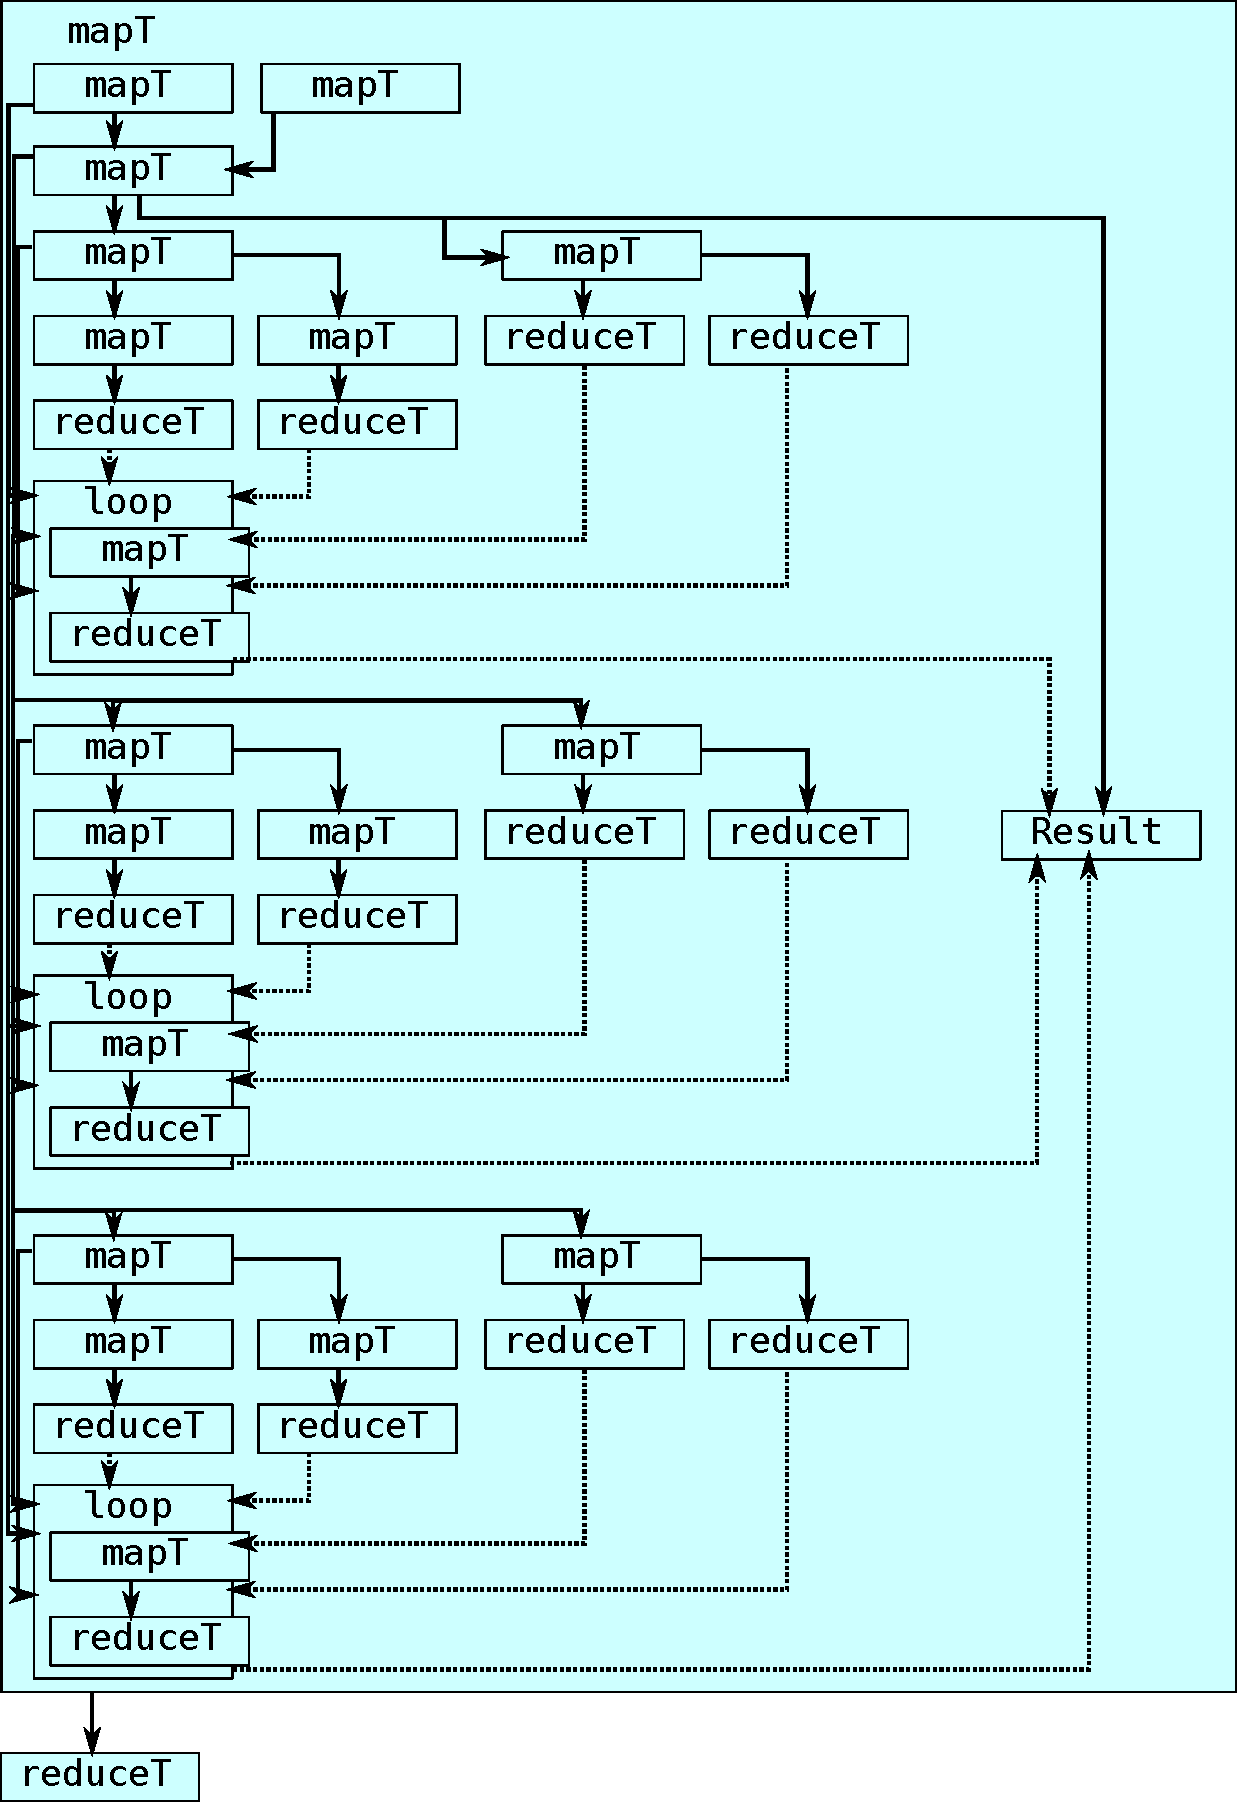
\includegraphics[width=9.6cm]{img/CalibLexiFi-unfused.pdf}
\end{center}
\caption{R0 benchmark dataflow, before optimisation}
\label{fig:r2-dataflow-unfused}
\end{figure}

\begin{figure}
\begin{center}
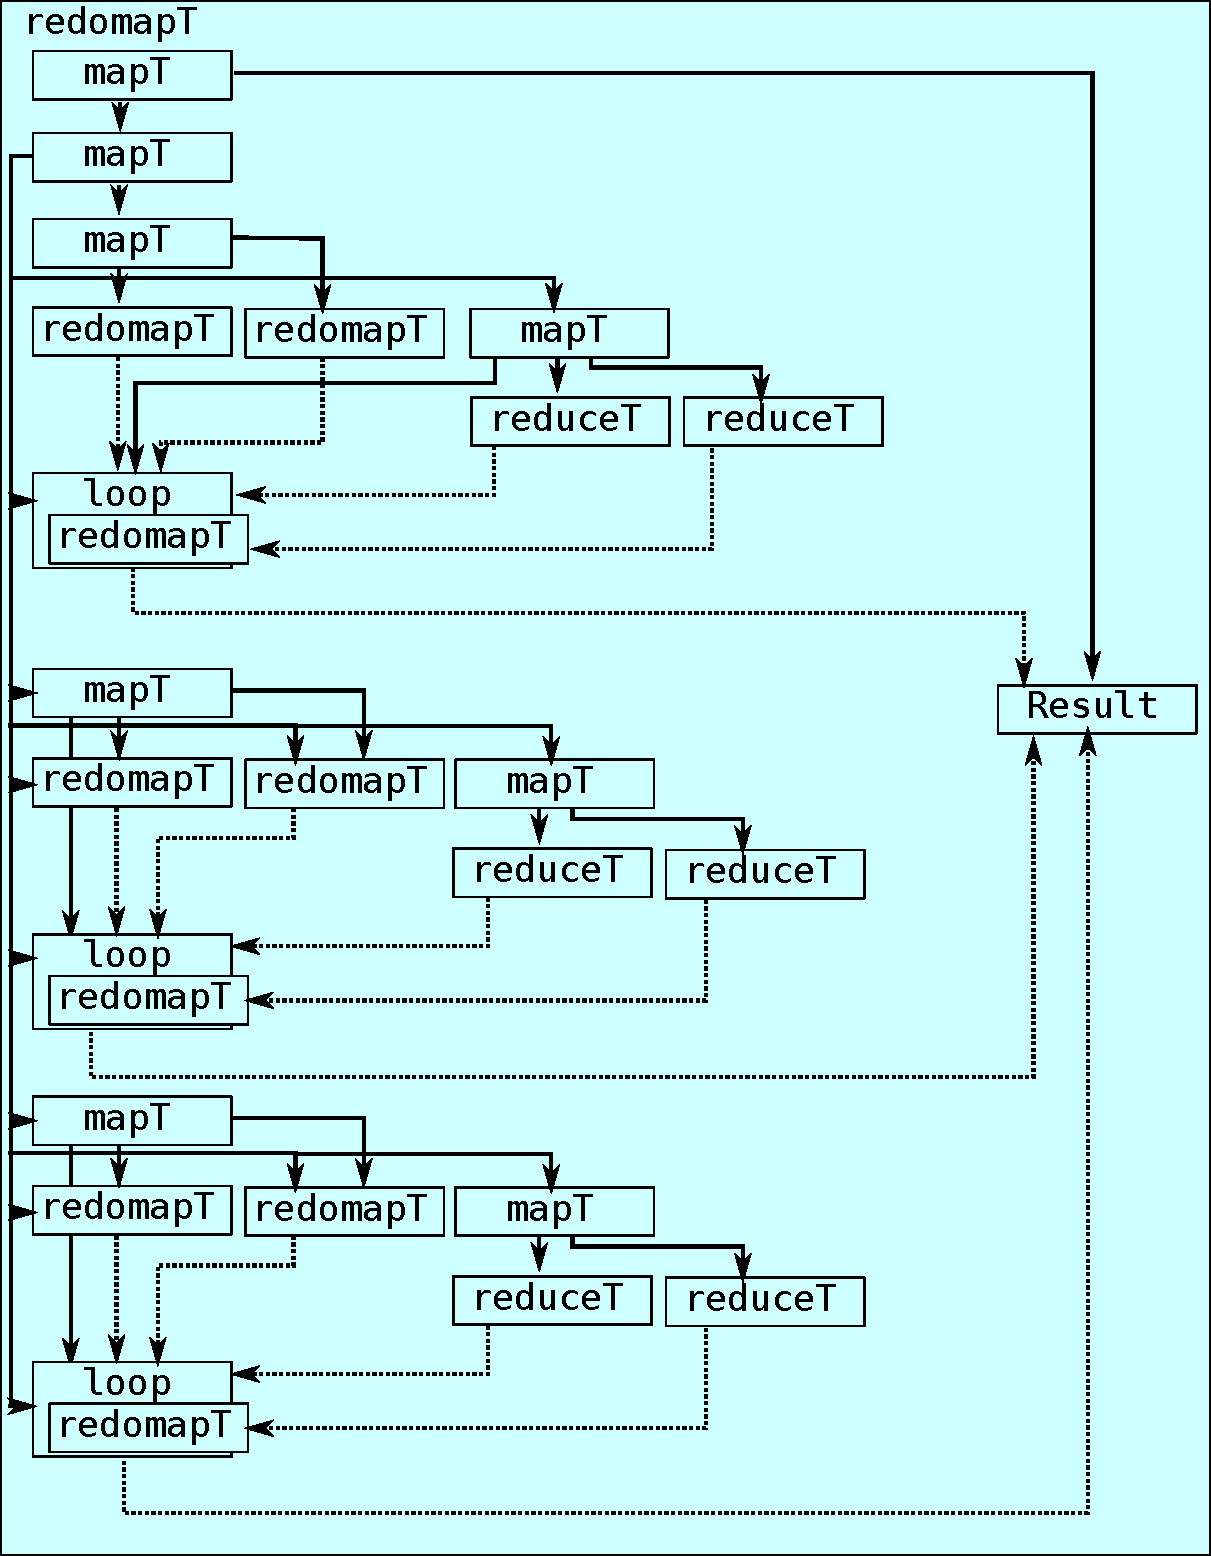
\includegraphics[width=9.6cm]{img/CalibLexiFi-fused.pdf}
\end{center}
\caption{R0 benchmark dataflow, after optimisation}
\label{fig:r2-dataflow-fused}
\end{figure}

\section{Runtime results}
\label{sec:runtime-results}

The resulting programs were compiled with GCC 4.8.2 using maximum
optimisation (\texttt{-O3}) on an Intel Core i7-2630QM CPU running at
2.00GHz.  Each program was executed one thousand times and the
run-times averaged.  The results are shown on \cref{fig:speedups}

\begin{figure}
\begin{center}
\begin{tabular}{l|c|c|c}
& \textbf{R0} & \textbf{R1} & \textbf{R2} \\
\textbf{Unoptimised} & 0.43018s & 0.09767s & 0.06179s \\
\textbf{Optimised}   & 0.29283s & 0.05681s & 0.04704s \\\hline
\textbf{Speedup}     & 46\%     & 71\%     & 31\%
\end{tabular}
\end{center}

\caption{Benchmark runtimes}

\label{fig:speedups}
\end{figure}


%%% Local Variables: 
%%% mode: latex
%%% TeX-master: "thesis.tex"
%%% End: 
